\documentclass[12pt]{article}
%\usepackage[english]{babel}
\usepackage{graphicx}
%\usepackage{framed}
%\usepackage[normalem]{ulem}
\usepackage{indentfirst}
\usepackage{amsmath,amsthm,amssymb,amsfonts}
\usepackage[italicdiff]{physics}
\usepackage[T1]{fontenc}
\usepackage{wrapfig}
\usepackage{lmodern,mathrsfs}
\usepackage[inline,shortlabels]{enumitem}
\setlist{topsep=2pt,itemsep=2pt,parsep=0pt,partopsep=0pt}
\usepackage[dvipsnames]{xcolor}
\usepackage[utf8]{inputenc}
%\usepackage[letterpaper, top=0.5in,bottom=0.2in, left=0.5in, right=0.5in, footskip=0.3in, includefoot]{geometry}
\usepackage[letterpaper,left=0.5in, right=0.5in,top=0.7in,bottom=1in,footskip=0.3in,includefoot]{geometry}
\usepackage[most]{tcolorbox}
\usepackage{tikz,tikz-3dplot,tikz-cd,tkz-tab,tkz-euclide,pgf,pgfplots}
\pgfplotsset{compat=newest}
\usepackage{multicol}
\usepackage[bottom,multiple]{footmisc} 
%\usepackage[backend=bibtex,style=numeric]{biblatex}
%\addbibresource{bibliography}
\usepackage{hyperref}
\usepackage[nameinlink]{cleveref} 
\usepackage[titletoc, toc, page]{appendix}


\newtheoremstyle{mystyle}{}{}{}{}{\sffamily\bfseries}{.\\}{ }{}
\newtheoremstyle{cstyle}{}{}{}{}{\sffamily\bfseries}{}{ }{\thmnote{#3}}

\theoremstyle{mystyle}{\newtheorem{definition}{Definition}[subsection]}
%\theoremstyle{mystyle}{\newtheorem{proposition}[definition]{Proposition}}
\theoremstyle{mystyle}{\newtheorem{theorem}[definition]{Theorem}}
%\theoremstyle{mystyle}{\newtheorem{lemma}[definition]{Lemma}}
%\theoremstyle{mystyle}{\newtheorem{corollary}[definition]{Corollary}}
\theoremstyle{mystyle}{\newtheorem*{remark}{Remark}}
%\theoremstyle{mystyle}{\newtheorem*{remarks}{Remarks}}
\theoremstyle{mystyle}{\newtheorem{example}{Example}[subsection]}
\theoremstyle{mystyle}{\newtheorem{examples}{Examples}[subsection]}
%\theoremstyle{definition}{\newtheorem*{exercise}{Exercise}}
\theoremstyle{mystyle}{\newtheorem{cthm}{}[subsection]}


\tcolorboxenvironment{definition}{boxrule=0pt,boxsep=0pt,colback={red!10},left=8pt,right=8pt,enhanced jigsaw, borderline west={2pt}{0pt}{red},sharp corners,before skip=10pt,after skip=10pt,breakable}
%\tcolorboxenvironment{proposition}{boxrule=0pt,boxsep=0pt,colback={Orange!10},left=8pt,right=8pt,enhanced jigsaw, borderline west={2pt}{0pt}{Orange},sharp corners,before skip=10pt,after skip=10pt,breakable}
\tcolorboxenvironment{theorem}{boxrule=0pt,boxsep=0pt,colback={blue!10},left=8pt,right=8pt,enhanced jigsaw, borderline west={2pt}{0pt}{blue},sharp corners,before skip=10pt,after skip=10pt,breakable}
\tcolorboxenvironment{example}{boxrule=0pt,boxsep=0pt,colback={Green!10},left=8pt,right=8pt,enhanced jigsaw, borderline west={2pt}{0pt}{Green},sharp corners,before skip=10pt,after skip=10pt,breakable}
\tcolorboxenvironment{examples}{boxrule=0pt,boxsep=0pt,colback={violet!10},left=8pt,right=8pt,enhanced jigsaw, borderline west={2pt}{0pt}{violet},sharp corners,before skip=10pt,after skip=10pt,breakable}
\tcolorboxenvironment{proof}{boxrule=0pt,boxsep=0pt,blanker,borderline west={2pt}{0pt}{CadetBlue!80!white},left=8pt,right=8pt,sharp corners,before skip=10pt,after skip=10pt,breakable}
\tcolorboxenvironment{remark}{boxrule=0pt,boxsep=0pt,blanker,borderline west={2pt}{0pt}{Cyan},left=8pt,right=8pt,before skip=10pt,after skip=10pt,breakable}
%\tcolorboxenvironment{remarks}{boxrule=0pt,boxsep=0pt,blanker,borderline west={2pt}{0pt}{Green},left=8pt,right=8pt,before skip=10pt,after skip=10pt,breakable}
%\tcolorboxenvironment{example}{boxrule=0pt,boxsep=0pt,blanker,borderline west={2pt}{0pt}{Black},left=8pt,right=8pt,sharp corners,before skip=10pt,after skip=10pt,breakable}
%\tcolorboxenvironment{examples}{boxrule=0pt,boxsep=0pt,blanker,borderline west={2pt}{0pt}{Black},left=8pt,right=8pt,sharp corners,before skip=10pt,after skip=10pt,breakable}
\tcolorboxenvironment{cthm}{boxrule=0pt,boxsep=0pt,colback={orange!10},left=8pt,right=8pt,enhanced jigsaw, borderline west={2pt}{0pt}{orange},sharp corners,before skip=10pt,after skip=10pt,breakable}



\usepackage[explicit]{titlesec}
\titleformat{\section}{\fontsize{24}{30}\sffamily\bfseries}{\thesection}{20pt}{#1}
\titleformat{\subsection}{\fontsize{16}{18}\sffamily\bfseries}{\thesubsection}{12pt}{#1}
\titleformat{\subsubsection}{\fontsize{10}{12}\sffamily\large\bfseries}{\thesubsubsection}{8pt}{#1}

\titlespacing*{\section}{0pt}{5pt}{5pt}
\titlespacing*{\subsection}{0pt}{5pt}{5pt}
\titlespacing*{\subsubsection}{0pt}{5pt}{5pt}

%\newcommand{\sectionbreak}{\clearpage} %Start every section on a new page
\newcommand{\tbf}[1]{\textbf{#1}}
\newcommand{\p}{\partial}
\newcommand{\id}{\mathrm{d}}
%\newcommand{\Disp}{\displaystyle}
%\newcommand{\qe}{\hfill\(\bigtriangledown\)}
%\DeclareMathAlphabet\mathbfcal{OMS}{cmsy}{b}{n}
%\setlength{\parindent}{0.2in}
%\setlength{\parskip}{0pt}
%\setlength{\columnseprule}{0pt}

\title{\huge\sffamily\bfseries General Relativity}
\author{\Large\sffamily Yucun Xie}
\date{\sffamily \today}

\begin{document}

\setlength{\abovedisplayskip}{3pt}
\setlength{\belowdisplayskip}{3pt}
\setlength{\abovedisplayshortskip}{0pt}
\setlength{\belowdisplayshortskip}{0pt}
\maketitle

%Custom colors for different environments
\definecolor{contcol1}{HTML}{72E094}
\definecolor{contcol2}{HTML}{24E2D6}
\definecolor{convcol1}{HTML}{C0392B}
\definecolor{convcol2}{HTML}{8E44AD}

\begin{tcolorbox}[
    title=Contents, fonttitle=\huge\sffamily\bfseries\selectfont,
    interior style={left color=contcol1!40!white,right color=contcol2!40!white},
    frame style={left color=contcol1!80!white,right color=contcol2!80!white},
    coltitle=black,top=2mm,bottom=2mm,left=2mm,right=2mm,drop fuzzy shadow,enhanced,breakable]
  \makeatletter
  \@starttoc{toc}
  \makeatother
\end{tcolorbox}


\newpage
\begin{tcolorbox}[
    title=Conventions, fonttitle=\large\sffamily\bfseries\selectfont,
    interior style={left color=convcol1!40!white,right color=convcol2!40!white},
    frame style={left color=convcol1!80!white,right color=convcol2!80!white},
    coltitle=black,top=2mm,bottom=2mm,left=2mm,right=2mm,drop fuzzy shadow,enhanced,breakable]
  \begin{enumerate}

    \item Greek index (e.g. $\alpha, \beta, \mu, \nu$) take value from \{0, 1, 2, 3\}.
          %\item Events denoted by cursive capitals  (e.g. $\mathscr{A}, \mathscr{B}, \mathscr{E}$).
    \item $(x^0, x^1, x^2, x^3) \equiv (t, x, y, z) \equiv x^{\alpha}$.
    \item Latin index (e.g. $ i, j, k$) take value from \{1, 2, 3\}.
    \item Natural units ($c=1$).
    \item Einstein summation convention. \[ds^2 = g_{\mu \nu} dx^{\mu} dx^{\nu}=
            \sum_{\mu=0}^{3} \sum_{\nu=0}^{3}g_{\mu \nu} dx^{\mu} dx^{\nu}\]
    \item Metric signature $(-, +, +, +)$.

  \end{enumerate}
\end{tcolorbox}

\newpage

%begin here ---------------------------------------------------------------------------------------------
\section{Differential Geometry}

\subsection{Manifolds}
Mathematically, spacetime is a \textbf{manifold}.

A manifold is a space that can be continuously (no hole, tear, etc.) covered by multiple coordinate charts.
For example, think about a sphere; we can stretch a membrane with the grid to cover it except for one point, then we can
use another membrane to cover that one point. The sphere is an example of a 2-D manifold, and the membrane is an example of a coordinate chart.
Informally, a manifold locally looks like \(\mathbb{R}^2\).
For example, the surface of the Earth is a 2-sphere $S^2$, but look at the ground around you; it seems flat.
\begin{definition}[Manifolds]
  An n-dimensional manifold is a mathematical structure consisting of
  \begin{enumerate}
    \item a set \(M\) of elements, called \textbf{points}.
    \item a countable family of subsets of \(M\), called \textbf{fundamental coordinate patches},
          such that the union of all of them is \(M\).
    \item a reversible mapping of each patch onto the unit volume of \(\mathbb{R}^n\). An n-tuple of numbers associated
          in this way are called the \textbf{coordinates} of each point.
  \end{enumerate}
  More formally, an n-dimensional manifold is a topological space that is locally homeomorphic to the n-dimensional Euclidean space.
  See the discussion of topological space for the definition of homeomorphism.\\
  If a manifold is differentiable for m times at each point, it is a \textbf{differentiable manifold}, denoted by \(C^m\).
  If a manifold is infinitely differentiable at each point, denote by \(C^\infty\), called a smooth manifold.\\
  A coordinate system (also called a chart) is n labels uniquely with each point of an n-dimensional manifold through a one-to-one mapping from
  $\mathbb{R}^n$ to $M$.\\
  Generally, more than one chart is required to cover the entire manifold, which is called \textbf{atlas}.
  %An n-dimensional manifold is a set that can be parameterized continuously by n independent real coordinates for each point.
\end{definition}
Differential geometry, as the name suggests, is geometry on differential manifolds.

Manifolds are very basic structures, but they support the following things on it.
\begin{enumerate}
  \item saclar field: \(\phi(x)\)
  \item curves: \(x^{\mu}(\lambda)\)
  \item surfaces: \(x^{\mu}(\lambda_1, \lambda_2)\)
  \item tangent vector and dual vector.
  \item tangent space and cotangent space.
\end{enumerate}

\subsubsection{Vector and Dual Vector}
At each point $P$ of an n-dimensional differentiable manifold, there is an n-dimensional vector space
which basis is defined by directional derivative at $P$ for curves passing through $P$.
This vector space is called \textbf{tangent space}. This space contains all \textbf{vectors} at point $P$.
There is also another vector space whose basis is defined by evaluating the gradient of the scalar function at $P$.
This space is called \textbf{cotangent space}, which contains all \textbf{dual vectors} at point $P$.\\
Vectors and dual vectors are local to a point.\\
Set of all tangent spaces in a manifold form a \textbf{tangent bundle}, and the set of all cotangent spaces on a manifold
form a \textbf{cotangent bundle}. They are an example of \textbf{fiber bundle}.\\
A fiber bundle is a manifold that is locally the cartesian product of base space and fiber space but not globally.\\
There is no definite way to transport a vector from one point to another on a manifold
because there is no relation between the tangent space at each point. To achieve this,
we need to impose an additional structure into the manifold, which is called \textbf{connection}.


\subsubsection{Maps Between Manifolds}
@TODO
pullback
pushforward


\subsection{Tensor}
A tensor is a quantity that has the same form in all coordinate systems.
Tensor does not have components naturally, but when we choose a specific coordinate system, we can write down its components.
Tensor has \textbf{Covariance}, which means it follows a specific transformation law.

\subsubsection{Tensor Notation}
A tensor with \(k\) upper indices and \(l\) lower indices
\[T^{\mu^1 \mu^2 \mu^3 \cdots \mu^k}_{\nu^1\nu^2\nu^2\cdots \nu^l}\]
is the cartesian product of k vectors and l dual vectors. Which map k dual vectors and l vectors to a real number.
\textbf{Cartesian product} $X \times Y$ is a set of all possible ordered pairs of the element one from $X$ and one from $Y$.

\subsubsection{Tensor Transformation Law}
When we change the coordinate system, tensor components transform following \textbf{tensor transformation law}.
\begin{definition}[Tensor transformation law]
  Tensor components in new coordinate system \((\alpha'\beta'\mu'\nu'\cdots)\) can be express as
  \[T^{\alpha'\beta'\cdots}_{\mu'\nu'\cdots} =
    \frac{\partial x^{\mu}}{\partial x^{\mu'}}\frac{\partial x^{\nu}}{\partial x^{\nu'}}\frac{\partial x^{\alpha'}}{\partial x^{\alpha}}
    \frac{\partial x^{\beta'}}{\partial x^{\beta}} \cdots
    T^{\alpha\beta\cdots}_{\mu\nu\cdots}\]
\end{definition}
Each upper indices is covariance with coordinate transform; each lower indices is contravariance with coordinate transform.
If some quantity obeys the tensor transformation law, it is a tensor. If a tensorial equation is held in one coordinate system,
it is held in all coordinate
system because both sides follow the same law to transform.

\subsubsection{Exterior Calculus}
A covariant totally antisymmetric rank \((0,p)\) tensor is called differential \(p\)-form. This is the reason why a dual vector is sometimes called 1-form.
We can generate new differential forms by taking the antisymmetric part of the tensor product, which is called \textbf{wedge product}.
\begin{example}
  The wedge product of two one form is \[(A\wedge B)_{\mu\nu}= 2A_{\left[\mu\right.}B_{\left.\nu\right]}\]
\end{example}
The \textbf{exterior derivative} can generate \(p+1\)-form from \(p\)-form.
\begin{definition}[Exterior derivative]
  Exterior derivative of a \(p\)-form \(A\) is defined as the following.
  \[dA = (p+1)\partial_{\left[\mu_1\right.}A_{\left.\mu_2\mu_3\cdots\mu_{p+1}\right]}\]
\end{definition}
A differential \(p\)-form \(A\) is \textbf{closed} if \(dA =0\), and \textbf{exact} if exist another differential form which \(dB = A\).
We see that definition of the exterior derivative does not require any additional structure.
The reason for defining differential form is that we can have derivative and integral without the help of additional structure on the manifold.

\subsection{Affine Connection}
Recall that we cannot transform vectors from one point to another on a manifold
because we miss the relation between tangent space at each point. So we introduce an additional structure called \textbf{connection}.
The connection is an additional structure that connects the tangent space on each point of a manifold.
There is no naturally defined connection on a manifold; we have to define one. Therefore connection on a manifold is not unique.
In general relativity, our spacetime manifold equipped with a metric-compatible, torsion-free connection is called \textbf{affine connection}.
Connection coeffienct in a coordinate system is express as \textbf{Christoffel symbol} \(\Gamma^{\lambda}_{\alpha\beta}\).\\
In general, a manifold with connection is a manifold allowing \textbf{parallel transport} of vectors.

\subsubsection{Covariant Derivative}
The partial derivative is not covariance; we are looking for another kind of differentiation that is covariant.
Here let me show that partial derivative, not covariance, and then construct a covariant one that we can apply to our curved spacetime.
\begin{align*}
  \begin{split}
    A_{\mu,\nu} &= \frac{\partial A_{\mu}}{\partial x^{\nu}} = \frac{\partial}{\partial x^{\nu}}
    \left( A_{\mu}\frac{\partial x^{\alpha}}{\partial x^{\mu}}\right)\\
    &= \frac{\partial A_\alpha}{\partial x^{\nu}}\frac{\partial x^{\alpha}}{\partial x^{\mu}}+
    A_{\alpha} \frac{\partial^2 x^{\alpha}}{\partial x^{\mu} \partial x^{\nu}}\\
    &= A_{\alpha,\beta}\frac{\partial x^{\beta}}{\partial x^{\nu}}\frac{\partial x^{\alpha}}{\partial x^{\mu}} +
    \underbrace{A_{\alpha} \frac{\partial^2 x^{\alpha}}{\partial x^{\mu} \partial x^{\nu}}}_\text{Not a tensor}
  \end{split}
\end{align*}\\
By using the connection coefficient below, which is also not a tensor, we can eliminate the none tensorial part of the partial derivative.
Which is defined as follows.
\begin{example}
  The covariant derivative of the dual vector.
  \[A_{\mu;\nu} = A_{\mu,\nu} - \Gamma^{\lambda}_{\mu\nu}A_{\lambda}\]
\end{example}

This is called \textbf{covariant derivative}, two non-tensorial parts added together to form a tensor.

\begin{proof}
  Here is proof shows that connection is not a tensor by show connection does not obey the tensor transformation law.
  \begin{align*}
    \begin{split}
      \nabla_{\beta'}e_{\alpha'} & = \Gamma^{\gamma'}_{\alpha'\beta'}e_{\gamma'} \\
      &= \frac{\partial x^{\beta}}{\partial x^{\beta'}}\nabla_{\beta}(\frac{\partial x^{\alpha}}{\partial x^{\alpha'}}e_{\alpha})\\
      &= \frac{\partial x^{\beta}}{\partial x^{\beta'}}
      (\frac{\partial}{\partial x^{\beta}}\frac{\partial x^{\alpha}}{\partial x^{\alpha'}}e_{\alpha}
      + \frac{\partial x^{\alpha}}{\partial x^{\alpha'}} \Gamma ^{\gamma}_{\alpha\beta} e_{\gamma})\\
      &= \frac{\partial x^{\beta}}{\partial x^{\beta'}}
      \frac{\partial}{\partial x^{\beta}}\frac{\partial x^{\alpha}}{\partial x^{\alpha'}}e_{\alpha}
      + \frac{\partial x^{\beta}}{\partial x^{\beta'}}
      \frac{\partial x^{\alpha}}{\partial x^{\alpha'}} \Gamma ^{\gamma}_{\alpha\beta} e_{\gamma}\\
      &= \frac{\partial x^{\beta}}{\partial x^{\beta'}}
      \frac{\partial}{\partial x^{\beta}}\frac{\partial x^{\alpha}}{\partial x^{\alpha'}}\frac{\partial x^{\gamma'}}{\partial x^{\alpha}}e_{\gamma'}
      + \frac{\partial x^{\beta}}{\partial x^{\beta'}}
      \frac{\partial x^{\alpha}}{\partial x^{\alpha'}} \frac{\partial x^{\gamma'}}{\partial x^{\gamma}} \Gamma ^{\gamma}_{\alpha\beta}  e_{\gamma'}\\
    \end{split}
  \end{align*}
  \\
  which yield \[\Gamma^{\gamma'}_{\alpha'\beta'} = \frac{\partial x^{\beta}}{\partial x^{\beta'}}
    \frac{\partial}{\partial x^{\beta}}\frac{\partial x^{\alpha}}{\partial x^{\alpha'}}\frac{\partial x^{\gamma'}}{\partial x^{\alpha}}
    + \frac{\partial x^{\beta}}{\partial x^{\beta'}}
    \frac{\partial x^{\alpha}}{\partial x^{\alpha'}}
    \frac{\partial x^{\gamma'}}{\partial x^{\gamma}} \Gamma ^{\gamma}_{\alpha\beta}\]
  There is an extra term in the transformation of connection, so the connection is not a tensor.
\end{proof}
Our connection is metric compatible and torsion-free, which mean \[g_{\mu\nu;\alpha} = 0\] and\[S_{\mu\nu} = \Gamma_{[\mu\nu]}^{\lambda} = 0 \]
Where \(S_{\mu\nu}\) is the torsion tensor.

\subsubsection{Parallel Transport}
Recall we defined connection to allow us to transport vectors on the manifold.
For \textbf{parallel transport} a vector, we want each infinitesimal step of transport to maintain the vector parallel.
Which required \textbf{intrinsic derivative} to vanish.\[\frac{DV^{\mu}}{D\lambda} =
  \frac{dV^{\mu}}{d\lambda}+ \Gamma^{\mu}_{\alpha\nu}V^{\alpha}\frac{dx^{\nu}}{d\lambda} = 0\]
\(\lambda\) is \textbf{affine parameter}, which is the parameter along the curve.

\subsection{Metric Space}
Now, in addition to affine connection, we want a structure allowing measurement of distance on the manifold.
The \textbf{metric space} is a kind of space with the notion of distance.
\begin{definition}[Riemannian manifold]
  A Riemannian manifold is a manifold with a connection and equipped with a symmetric \textbf{metric tensor} \(g_{\mu\nu}\).
  which distance \(ds\) between two points with displacement \(dx^{\mu}\) is defined as the following.
  \[ds^2 \equiv g_{\mu \nu} dx^{\mu} dx^{\nu}\]
\end{definition}
The metric tensor is one of the most important tensors in general relativity,
which directly lead to all spacetime structures.
\begin{example}
  The connection coefficient can be directly calculated from the metric tensor.
  \[\Gamma_{\mu\nu}^{\lambda} = \frac{1}{2}g^{\lambda\sigma}(\partial_{\mu}g_{\nu\sigma}+ \partial_{\nu}g_{\sigma\mu}
    - \partial_{\sigma}g_{\mu\nu})\]
\end{example}
In general relativity, proper time equates to distance in the timelike direction \(d\tau^2 = - ds^2\).

\subsubsection{Riemann Tensor}
We have everything we need to define the \textbf{curvature}. Think about transporting a vector \(V^\rho\)
around an infinitesimal loop on a curved manifold, the loop is defined by two vectors \(dA^\mu\) and \(dB^\nu\).
Then, the change on \(V^\rho\) can be express as \[\delta V^\rho = R^{\rho}_{\ \sigma\mu\nu}V^{\sigma}dA^{\mu}dB^{\nu}\]

\begin{definition}[Riemann tensor]
  \(R^{\rho}_{\ \sigma\mu\nu}\) is known as \textbf{Riemann curvature tensor}, or just Riemann tensor,
  can be express through connection coeffienct: \[R^{\rho}_{\ \sigma\mu\nu} =
    \partial_{\mu} \Gamma^{\rho}_{\nu\sigma} -
    \partial_{\nu} \Gamma^{\rho}_{\mu\sigma} +
    \Gamma^{\rho}_{\mu\lambda}\Gamma^{\lambda}_{\nu\sigma} -
    \Gamma^{\rho}_{\nu\lambda}\Gamma^{\lambda}_{\mu\sigma}
  \]
\end{definition}
There is some property in the Riemann tensor.

\begin{cthm}
  \begin{align*}
    \begin{split}
      R_{\alpha\beta\mu\nu} &= -R_{\beta\alpha\mu\nu}\\
      R_{\alpha\beta\mu\nu} &= -R_{\alpha\beta\nu\mu}\\
      R_{\alpha\beta\mu\nu} &= R_{\mu\nu\alpha\beta}\\
      R_{\alpha\beta\mu\nu} + R_{\alpha\nu\beta\mu} + R_{\alpha\mu\nu\beta} &= 0 \\
      \nabla_{\left[ \lambda \right.} R_{\left.\alpha\beta \right] \mu\nu} &= 0 \\
    \end{split}
  \end{align*}
  The last line above is called \textbf{Bianchi identity}.
\end{cthm}

\begin{definition}[Ricci tensor]
  From the Riemann tensor, we can construct a symmetric rank-2 tensor, \textbf{Ricci tensor}
  by contract first and the third indices of the Riemann tensor.
  \[R_{\mu\nu} = R_{\nu\mu} = R^{\lambda}_{\ \mu\lambda\nu}\]
  Furthermore, we can take the trace of the Ricci tensor to get \textbf{Ricci scalar} or scalar curvature.
  \[R = g^{\mu\nu}R_{\mu\nu}\]
\end{definition}

We can recover the Riemann tensor from scalar curvature through metric tensor.
\[R_{\alpha\beta\mu\nu} = \frac{R}{2}(g_{\alpha\mu}g_{\beta\nu}-g_{\beta\mu}g_{\alpha\nu})\]

From Bianchi identity \(\nabla_{\left[ \lambda \right.} R_{\left.\alpha\beta \right] \mu\nu} = 0\),
we can find that \[\nabla_{\mu}(R^{\mu\nu}-\frac{1}{2}g^{\mu\nu}R) = 0\]
We see the divergence of this tensor vanish. Therefore, we define a new tensor named \textbf{Einstein tensor},
\[G^{\mu\nu}=R^{\mu\nu}-\frac{1}{2}g^{\mu\nu}R. \]
The trace-free part of the Riemann tensor is called \textbf{Weyl tensor} and can be defined as follows.

\begin{definition}[Weyl tensor]
   @TODO
  \[C_{\rho\sigma\mu\nu} = \]
\end{definition}
\subsection{Geodesics}

\textbf{Geodesic} is the generalization of the straight line in curved spacetime, which is the trajectory of the inertially moving particle.
More specifically, geodesic is a path parallel-transport its own tangent vector.
Recall our equation of parallel transport, \(\frac{DV^{\mu}}{D\lambda} =
\frac{dV^{\mu}}{d\lambda}+ \Gamma^{\mu}_{\alpha\nu}V^{\alpha}\frac{dx^{\nu}}{d\lambda} = 0\) and replace \(V\)
by tangent vector of the path \(\frac{dx^{\mu}}{d\lambda}\). We get
\[\frac{D}{D\lambda}\frac{dx^{\mu}}{d\lambda} =
  \frac{d}{d\lambda}\frac{dx^{\mu}}{d\lambda}+ \Gamma^{\mu}_{\alpha\nu}\frac{dx^{\alpha}}{d\lambda}\frac{dx^{\nu}}{d\lambda} = 0\]\\
This is famous \textbf{geodesic equation}, all path satisfy this equation is a geodesic.

\begin{definition}[Geodesic equation]
  
  \[\frac{d^2 x^{\mu}}{d\lambda^2}+ \Gamma^{\mu}_{\alpha\nu}\frac{dx^{\alpha}}{d\lambda}\frac{dx^{\nu}}{d\lambda} = 0\]
\end{definition}

Geodesic always maximized the proper time. Think about the twin paradox in special relativity; the twin stays on Earth and approximately moves alone geodesic,
but the twin travels away at the tuning point isn't move-alone geodesic.

\subsection{Killing Vector Field}
The symmetric property of spacetime is represented by \textbf{killing vector field}.
\begin{definition}[Killing vector fields]
  A killing vector \(K\) satisfy the \textbf{killing equation}:
  \[\mathcal{L}_{K}g_{\mu\nu}= 0\]\\
  where \(\mathcal{L}_{K}\) is the Lie derivative alone \(K\). For the definition of Lie derivative, refer to the appendix.
\end{definition}


\subsection{Geodesic Deviation}
\newpage
\section{Gravitation}

Our spacetime is not simply a Riemannian manifold but a \textbf{pseudo-Riemannian manifold}, which is a more general Riemannian manifold.
Riemannian manifold requires the metric tensor to be positive definite, which means all eigenvalue of the metric tensor is positive.
For the pseudo-Riemannian manifold, the metric eigenvalue can be either positive or negative, called indefinitely.

\begin{remark}
  The eigenvalue of the metric can not be zero; if an eigenvalue is zero, the metric will degenerate and have no inverse.
\end{remark}

More specifically, our spacetime is \textbf{Lorentzian manifold}, which is a pseudo-Riemannian manifold with only one negative eigenvalue.
The Lorentzian manifold allows us to classify tangent vectors into timelike, spacelike, and lightlike.

\subsection{Equivalence Principle}
\begin{definition}[Weak equivalence principle]
The weak equivalence principle is stated as follow:
  \begin{enumerate}
    \item Inertial mass is defined through Newton's second law, \(m = F/a\).
    \item Gravitational mass is defined through Newton's law of gravity \(m = Fr^2/GM\).
  \end{enumerate}
\end{definition}

There are two equivalence principles, the weak equivalence principle, and the strong equivalence principle
(or Einstein's equivalence principle). Weak Principle of Equivalence state that inertial mass is always equal to gravitational mass.
Einstein extended this idea to a stronger statement, which is \textbf{Strong Equivalence Principle}.
Which state that observer is unable to distinguish acceleration and gravitational field by local experiment.
This leads to the idea of \textbf{local inertial frame}, which is correspondence to the property of manifold (local flatness).
With the equivalence principle, we can explain the deflection of light and gravitational redshift in the gravitational field.

\textbf{General Covariance Principle} state that if a tensorial equation hold in a gravitational field yield that

\begin{enumerate}
  \item hold in the absence of gravity.
  \item holds under a coordinate transformation.
\end{enumerate}
Therefore, we can write our classical equations in tensorial form, then they will hold in general relativity.

\begin{example}
  Tensorial Maxwell's equations:
  \begin{align*}
    \begin{split}
      \nabla_{\mu}F^{\nu\mu} &= J^{\nu}\\
      \nabla_{\left[ \mu\right.}F_{\left. \nu\lambda \right]} &= 0
    \end{split}
  \end{align*}
\end{example}

In general, we can replace the partial derivative with the covariant derivative and replace the flat spacetime metric by \(g_{\mu\nu}\),
then it will be valid in curved spacetime.



\subsection{Einstein's Equation}
From the Poisson equation for Newtonian potential:
\[\nabla^2 \phi = 4 \pi G \rho\]
To make a relativistic version of this equation, we can replace the gravitational potential with the metric and the mass density with the energy-momentum tensor.
\[\nabla^2 g_{\mu\nu} = c T_{\mu\nu}\]
But the second derivative of the metric vanished by metric compatibility of connection. Therefore we want something constructed from the metric's second derivative that does not vanish.
Riemann tensor fits this requirement but does not have the right number of indices, so we can use the Ricci tensor.
\[R_{\mu\nu} = c T_{\mu\nu}\]
But, this still doesn't seem right; recall the conservation of energy, \(\nabla^{\mu}T_{\mu\nu} = 0\); the Ricci tensor does not fit this requirement.
We need a rank two tensor that is conserved and fits the requirement above. We do have one, the Einstein tensor:
\[\nabla^{\mu}G_{\mu\nu} = 0\]
Then our equation read \[R_{\mu\nu} -\frac{1}{2}Rg_{\mu\nu} = cT_{\mu\nu}\]
This is the famous Einstein field equation. We can recover the constant by requiring the equation back to the Newtonian limit.

To recover Newtonian gravity, impose the following boundary conditions on the field equation:
\begin{enumerate}
  \item Weak field (\(g_{\mu\nu} = \eta_{\mu\nu} + h_{\mu\nu}\) which \(\left|h_{\mu\nu}\right| \ll 1\))
  \item Stationary (time translational symmetry).
  \item Low speed (reduce special relativity to Newtonian mechanics).
\end{enumerate}

In this limit, the energy-momentum tensor simply \(T_{00} = \rho\) and all other components vanish.
Rearrange Einstein equation, we get \(R_{\mu\nu} = c\left( T_{\mu\nu} - \frac{1}{2}Tg_{\mu\nu} \right)\),
plug \(T_{00} = \rho\) in to field equation, we get \(R_{00}=\frac{1}{2}c\rho\). \\
From the Riemann tensor in week field limit, we can see that \(R_{00}=-\frac{1}{2}\nabla^2 h_{00}\);
Compared to the Poisson equation of Newtonian gravity, we know that \(c = 8\pi G\).
\begin{cthm}
  Einstein field equation.
  \[R_{\mu\nu} -\frac{1}{2}Rg_{\mu\nu} = 8\pi GT_{\mu\nu}\]
\end{cthm}
\newpage
\section{Relativistic Star}

\subsection{Schwarzschild Solution}

The first exact solution to Einstein's equation by Karl Schwarzschild is named \textbf{Schwarzschild solution},
which is the exterior solution to a spherical star.
This solution is solved by imposing the following boundary conditions:

\begin{enumerate}
  \item Static, which means completely independent of time. More formally, the metric tensor satisfies time translational symmetry and time reversal symmetry.
  \item Vacuum, which means the solution is only valid outside the star, implying vanish of the energy-momentum tensor.
        This means the solution is not valid in the interior of the star.
  \item Spherical symmetry, which means that, given a radius, the spacetime should be the same.
\end{enumerate}

\begin{cthm}
  The line element takes the form
  \[ds^2 = -\left(1 - \frac{r_\mathrm{s}}{r} \right)\,dt^2 + \left(1-\frac{r_\mathrm{s}}{r}\right)^{-1} \,dr^2 + r^2 d\Omega^2\]\\
  which \(r_\mathrm{s} = 2GM\) and \(d\Omega^2 = \left(d\theta^2 + \sin^2\theta \, d\phi^2\right)\).
\end{cthm}
From this line element, we can notice a few properties of the Schwarzschild metric.
\begin{enumerate}
  \item Singularity at \(r = 2GM\) and \(r = 0\).
  \item Change of sign of \(g_{tt}\) and \(g_{rr}\) at \(r = 2GM\).
  \item Recover to Newtonian gravity at the Newtonian limit.
  \item Asymptotic flatness.
\end{enumerate}

The surface at \(r = 2GM\) is known as \textbf{Schwarzschild horizon}; this radius is known as the Schwarzschild radius.
This led to the idea of the black hole, in which nothing can escape from the horizon (at least in the classical limit, we will see a later discussion of Hawking radiation). 

We can calculate the timelike geodesic from the metric, which implies planetary motion in general relativity, leading to the famous result of the precession of the perihelion of Mercury.
We are also able to calculate the deflection of light by calculating lightlike geodesic from metric; this leads to the effect of \textbf{gravitational lensing}.

\subsubsection{Interior Solution}

Recall the Schwarzschild solution is only valid outside the spherical star, not the interior, so there is no singularity and horizon on our Earth.
The interior solution can be solved by approximating the star by energy-momentum tensor of perfect fluid \(T_{\mu\nu} = (\rho + p)U_\mu U_\nu + pg_{\mu\nu}\),
and match the exterior solution at the boundary. The interior solution of a spherical star read \[ds^{2} =
  -\frac{1}{4} \left( 3 \sqrt{1-\frac {r_s}{r_g}}-\sqrt{1-\frac{r^2 r_s}{r_g^3}} \right)^2 dt^2 +
  \left( 1-\frac{r^2 r_s}{r_g^3} \right)^{-1} dr^2 + r^2 \mathrm{d}\Omega^2\]
Where \(r_{g}\) is the radius of the surface.

\subsubsection{Black hole}

\subsubsection{Maximal Extension}

\subsection{Kerr Solution}
Kerr solution is the vacuum solution to the axisymmetry rotating star by applying the following conditions to the Einstein equation.
\begin{enumerate}
  \item Stationary, which metric tensor satisfies time translational symmetry.
  \item Vacuum, which means the solution is only valid for the region outside the star, implying vanish of the energy-momentum tensor.
        This means the solution is not valid in the interior of the star.
  \item Axissymmetry, which means for given \(r\) and \(\theta\), metric components are the same.
\end{enumerate}
Kerr metric can be expressed in Boyer-Lindquist coordinates.
\begin{cthm}
  \[ds^{2} =
    -\left( 1 - \frac{2GM\; r}{\Sigma} \right) dt^{2} + \frac{\Sigma}{\Delta} dr^{2} + \Sigma d\theta^{2}
  \] \[+\left(r^2+ a^2 + \frac{2GM\; r a^{2}}{\Sigma} \sin^{2}\theta \right) \sin^{2}\theta \ d\phi^{2}\]
  \[ -\frac{4GM\; ra \sin^{2} \theta}{\Sigma} dt \, d\phi\]\\
  Where \(a = \frac{J}{Mc}\), \(\Sigma = r^{2} + a^{2} \cos^{2}\theta\), and \(\Delta = r^{2} - r_{s} r + a^{2}\).
\end{cthm}

\subsubsection{Dragging of Inertial Frame}

\subsubsection{Ergosphere}

\subsubsection{Penrose Process}
\newpage
\section{Gravitational Radiation}
\subsection{Linearized Gravity}
When the gravitational field is weak, the metric takes the following form:\[g_{\mu\nu} = \eta_{\mu\nu} + h_{\mu\nu} \]
which we treat the gravitational field as a perturbation of flat spacetime metric.
\subsection{Gravitational Wave}
\subsubsection{Effect of Gravitational Wave on matter}
\subsubsection{Source of Gravitational Wave}

\newpage

\section{Cosmology}
\subsection{Roberson-Walker Metric}
\subsection{Friedmann Equation}
\subsection{Inflation}

\newpage
\appendix


\addcontentsline{toc}{section}{Appendix~}

\section{Special Relativity}

\subsection{Spacetime}
In special relativity, we discard the absolute concept of time; in contrast to Newton, there is no preferred reference frame
and time is one of the coordinates.
Now we have a 4-dimensional \textbf{spacetime}. Our discussion is focused on the inertial coordinate system.
\begin{definition}[Inertial coordinate]
  The coordinate system must satisfy three properties to be considered inertial coordinate:
  \begin{enumerate}
    \item The distance between two points is independent of time.
    \item The clocks at every points ticking off time coordinate $t$ at the same rate.
    \item The geometry of space is always flat.
  \end{enumerate}
  It is a coordinate system without acceleration.
\end{definition}

\begin{figure}[ht]
  \begin{center}
    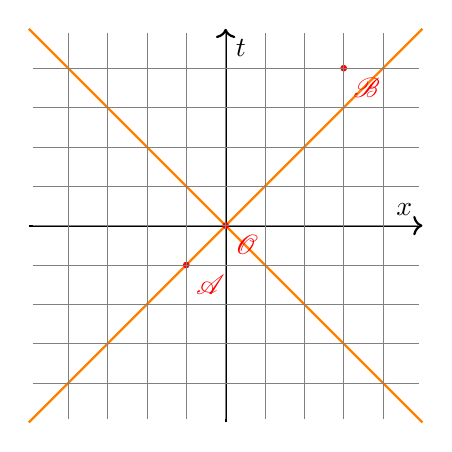
\begin{tikzpicture}[scale = 0.5]
      %\draw[orange, thick] (-5,0) -- (5,0);
      %\draw[orange, thick] (0,-5) -- (0,5);

      \draw[thick,->] (0,-5) -- (0,5) node[anchor=north west] {$t$};
      \draw[orange, thick] (-5,-5) -- (5,5);
      \draw[orange, thick] (-5,5) -- (5,-5);
      \draw[thick,->] (-5,0) -- (5,0) node[anchor=south east] {$x$};
      \filldraw[red] (-1,-1) circle (2pt) node[anchor=north west] {$\mathscr{A}$};
      \filldraw[red] (0,0) circle (2pt) node[anchor=north west] {$\mathscr{O}$};
      \filldraw[red] (3,4) circle (2pt) node[anchor=north west] {\(\mathscr{B}\)};
      \draw[step=1cm,gray,very thin] (-4.9,-4.9) grid (4.9,4.9);

    \end{tikzpicture}
    \caption[]{two events with coordinate $(-1, -1, 0, 0)$ and $(4, 3, 0, 0)$. The orange line is light's worldline.}
  \end{center}
\end{figure}

The event in 4-D spacetime is defined by a set of coordinates \((t, x, y, z)\).
For simplicity, we assume those events have $y=0, z=0$ so that we can draw a 2D graph to represent them.\\
Analog to Euclidean geometry, just like the euclidean distance \(\Delta l^2 = \Delta x^2 + \Delta y^2 + \Delta z^2\), we define the
\textbf{spacetime interval} $\Delta s^2 = - \Delta t^2 + \Delta x^2 + \Delta y^2 + \Delta z^2$.

\begin{remark}\leavevmode
  There are a lot of different conventions to define the sign of the spacetime interval; here, we use the popular one \((-,+,+,+)\).
\end{remark}
\begin{example}\leavevmode % This is needed to start the list in the next line so it won't be misaligned
  Interval for the two events in Figure 1 is $\Delta s^2 = - \Delta t^2 + \Delta x^2 + \Delta y^2 + \Delta z^2 = -9$.
\end{example}
The universality speed of light means that $\frac{\Delta r}{\Delta t} = \frac{\sqrt{\Delta x^2+ \Delta y^2 + \Delta z^2}}{\Delta t}=1$
are always hold, then we can then write the interval
$\Delta s^2 = - \Delta t^2 + \Delta x^2 + \Delta y^2 + \Delta z^2 = 0$. This experimental fact yield all laws of special relativity.
%Due to the universal speed of light, the interval is an invariant change of inertial coordinate; this means that $\Delta s^2 =\Delta \bar{s}^2$ 
%which $\Delta \bar{s}^2$ is $\Delta s^2$ in another inertial coordinate system.\\
\\
When the interval $\Delta s^2$ is less than 0, we call the separation between events is \textbf{timelike};
When the interval $\Delta s^2$ is equal to 0, we call it \textbf{lightlike} or null;
When the interval $\Delta s^2$ is greater than 0, we call it \textbf{spacelike}.
%The $x^{\mu}=\{x^0,x^1,x^2,x^3\} =\{t, x, y, z\}$ is a set of coordinate.
If there is another coordinate system, which moves with speed \(v\) alone \(x\) direction of the original frame,
we can draw this frame like Figure 2 below.
\begin{figure}[ht]
  \begin{center}
    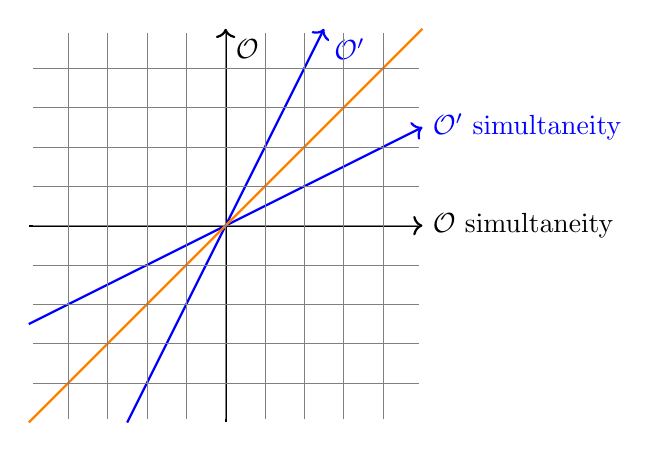
\begin{tikzpicture}[scale = 0.5]%Edit size here
      \draw[thick,->] (0, -5) -- (0, 5) node[anchor=north west] {$\mathcal{O}$};
      \draw[thick,->] (-5, 0) -- (5, 0) node[anchor=west] {$\mathcal{O}$ simultaneity};
      \draw[blue, thick,->] (-2.5, -5) -- (2.5, 5) node[anchor=north west] {$\mathcal{O}'$};
      \draw[blue, thick,->] (-5, -2.5) -- (5, 2.5) node[anchor=west] {$\mathcal{O}'$ simultaneity};
      \draw[orange, thick] (-5,-5) -- (5,5);
      \draw[step=1cm,gray,very thin] (-4.9,-4.9) grid (4.9,4.9);
    \end{tikzpicture}
    \caption[]{Frame \(\mathcal{O}'\) move alone x direction of \(\mathcal{O}\)}
  \end{center}
\end{figure}

\subsection{Fluid}

\newpage
\section{Classical Field Theory}
Classical field theory is something you are supposed to know for QFT but is never formally taught, so I give a brief overview here.
Field theory is very similar to Lagrangian mechanics; instead of the usual system,
we now have a spacetime-dependent \textbf{fields} \(\Phi^i(x^\mu)\) (the \(i\) here is not tensor index),
and the action becomes a \textbf{functional} of these fields. A functional is a ``function of function'', which map a function to a number,
note that the functional is not simply a composition function, which maps number to number. \par
In field theory, the Lagrangian is usually expressed as an integral over \textbf{Lagrange density},
which are a function of the fields and their derivative.
\begin{cthm}
  \[L=\int d^3x\;\mathcal{L}(\Phi^i,\partial_{\mu}\Phi^i)\]
\end{cthm}
Then the action
\begin{cthm}
  \[S=\int dt\;L = \int d^4x\;\mathcal{L}(\Phi^i,\partial_{\mu}\Phi^i)\]
\end{cthm}
By varying the action, just like what we did in classical mechanics, we can obtain the equation of motion of field:
\begin{cthm}
  \begin{align*}
    \delta S & = \int d^4x\left[\frac{\partial\mathcal{L}}{\partial \Phi^i}\delta\Phi^i+
    \frac{\partial\mathcal{L}}{\partial(\partial_\mu \Phi^i)}\partial_\mu (\delta\Phi^i)\right] \\
             & =\int d^4x\left[\frac{\partial\mathcal{L}}{\partial \Phi^i}-\partial_\mu
      \frac{\partial\mathcal{L}}{\partial(\partial_\mu \Phi^i)}\right]\delta\Phi^i
  \end{align*}
\end{cthm}
We have obtained the field version of \textbf{Euler-Lagrange equation}
\begin{cthm}
  \[\frac{\partial\mathcal{L}}{\partial \Phi^i}-\partial_\mu
    \frac{\partial\mathcal{L}}{\partial(\partial_\mu \Phi^i)}=0\]
\end{cthm}
Let's consider a simple example, the real scalar field \[\phi:\ x^{\mu} \rightarrow \mathbb{R}\].
The contribution of action are

\begin{enumerate}
  \item Kinetic term: \(\frac{1}{2}\dot{\phi}^2\)
  \item Gradient term: \(\frac{1}{2}(\nabla\phi)^2\)
  \item potential term: \(V(\phi)\)
\end{enumerate}
We could combine them into a Lorentz-invariant Lagrange density:
\begin{cthm}
  \[\mathcal{L}= \frac{1}{2}\eta^{\mu\nu}(\partial_{\mu}\phi)(\partial_{\nu}\phi)-V(\phi)\]
\end{cthm}
Apply the Euler-Lagrange equation; we then get the equation of motion:
\begin{cthm}
  \begin{align*}    & \eta^{\mu\nu}\partial_{\mu}\partial_{\nu}\phi+\frac{\mathrm{d}V(\phi)}{\mathrm{d}\phi} \\
              =\  & \square\phi+\frac{\mathrm{d}V(\phi)}{\mathrm{d}\phi}                                   \\
              =\  & 0
  \end{align*}
  Where \(\square\) is \textbf{d'Alembertian}.
\end{cthm}
\subsection{Klein-Gordon Field}
If the scalar field is massive, the potential \(V(\phi)=\frac{1}{2}m^2\phi^2\),
we obtained the \textbf{Klein-Gordon equation}:
\begin{cthm}
  \[(\square +m^2)\phi = 0\]
\end{cthm}
You will see this equation again and again in quantum field theory.
\begin{remark}
  The Klein-Gordon field could be analog to infinite many coupled infinitesimal harmonic oscillators,
  each ``mass'' is affected by neighboring springs and has its kinetic energy.

\end{remark}
\subsection{Noether's Theorem}
A Lagrangian may be invariant under some special type of transformation.
For example, a Lagrangian for a complex scalar field
\[\mathcal{L}= |\partial_\mu \phi|^2 -m^2|\phi|^2\]
is invariant under transformation \(\phi \rightarrow e^{i\alpha}\phi\).
We call this transformation a \textbf{symmetry} of the Lagrangian.
When the parameter of transformation (\(alpha\) for this case) can be taken infinitesimal,
we say this symmetry is \textbf{continuous}.
We can explicit see that \(\frac{\delta \mathcal{L}}{\delta \alpha}=0\).
\par By applying the Euler-Lagrange equation, we can deduce that \(\partial_\mu J_{\mu}=0\),
where \(J_{\mu}\) is defined as follow:
\begin{definition}
  \[J_{\mu}= \sum_n\frac{\partial \mathcal{L}}{\partial(\partial_\mu \phi_n)}\frac{\delta\phi_n}{\delta \alpha}\]\\
  \(J_{\mu}\) is known as \textbf{Noether current} or \textbf{conserved current}
\end{definition}

\begin{example}
  For the above complex scalar field, we can calculate the conserved current:
  \bigskip
  \begin{align*}
    J_{\mu}= & \sum_n\frac{\partial \mathcal{L}}{\partial(\partial_\mu \phi_n)}\frac{\delta\phi_n}{\delta \alpha} \\
    =        & \frac{\partial \mathcal{L}}{\partial(\partial_\mu \phi)}\frac{\delta\phi}{\delta \alpha}
    +\frac{\partial \mathcal{L}}{\partial(\partial_\mu \phi^*)}\frac{\delta\phi^*}{\delta \alpha}                 \\
    =        & -i\left[\phi\partial_\mu\phi^*-\phi^* \partial_\mu\phi\right]
  \end{align*}
  We can check that \(\partial_\mu J_{\mu}=0\) explicitly:
  \begin{align*}
    \partial_\mu J_{\mu}= & -i\left[\phi\square\phi^*-\phi^* \square\phi\right] \\
    =                     & 0
  \end{align*}
  Where we applied the equation of motion in the last step.
\end{example}
We call \(J_\mu\) conserved current because we can find conserved quantity by integral over its 0-component:
\begin{definition}
  \[Q=\int d^3x\;J_0\]
  Where the \(Q\) is called \textbf{conserved charge} or \textbf{Noether's charge}
\end{definition}[Conserved charge]
We say \(Q\) is conserved because
\begin{cthm}
  \[\partial_tQ=\int d^3x \; \partial_t J_0 = \int d^3x\;\vec{\nabla}\cdot \vec{J} = 0.\]
\end{cthm}
The above argument is called \textbf{Noether's theorem}.
\begin{theorem}[Noether's theorem]
  If a Lagrangian has a continuous symmetry,
  then exists a current associated with that symmetry that is 
  conserved when the equations of motion are satisfied.
\end{theorem}

\subsection{Energy-momentum Tensor}
The physics at spacetime point \(x\) should have same form at spacetime point \(y\),
this argument arises a symmetry called \textbf{specetime translational symmetry}.
By Noether's theorem, we can find the four conserved currents for this symmetry for an infinitesimal
spacetime translation \(\xi^\mu\):
\begin{cthm}
 \[T_{\mu\nu}=\sum_n \frac{\partial \mathcal{L}}{\partial(\partial_{\mu}\phi_n)}\partial_\nu\phi_n-g_{\mu\nu}\mathcal{L}\]
 
\(T_{\mu\nu}\) is called \textbf{energy-momentum tensor}.
\end{cthm}
Four conserved currents correspond to values of \(\nu\), and four conserved charges are energy and momentum.
We can see that the energy density is the 00-component of \(T_{\mu\nu}\).




%\section{Skipped proof}
\newpage
\section{Topological Space}
\newpage
\section{Lie Algebra}

\subsection{Lie Derivative}
Lie derivative is a more ``fundamental'' way to generalize derivative to a manifold than covariant derivative. \\
To see why it is more fundamental, consider the \textbf{Lie bracket}
\begin{definition}
  Lie bracket
  \bigskip
  \[\left[X, Y\right]^{\mu}= X^{\lambda}\nabla_{\lambda}Y^{\mu} - Y^{\lambda}\nabla_\lambda X^{\mu}\]\\
  It is easy to check that the above expression is equivalent to
  \(\left[X, Y\right]^{\mu}= X^{\lambda}\partial_{\lambda}Y^{\mu} - Y^{\lambda}\partial_\lambda X^{\mu}\).
\end{definition}

Lie bracket is a special kind of \textbf{Lie derivative}. The above expression is equivalent to
\(\mathcal{L}_{X}Y^{\mu}\). We see that the Lie derivative does not rely on affine connection.

The basic idea of Lie derivative is to use derivatives of an auxiliary vector field to
cancel the non-tensorial part of the partial derivative.

Let's go step by step to see how the Lie derivative work.

Consider a tensor on a manifold defined at point \(P\), it can be ``dragged'' to a nearby point \(Q\), alone
a curve of the congruence that generates by a vector field.

This step is called \textbf{Lie dragging}.

\newpage

\section{Penrose Diagram}

\newpage
\section{Scalar Tensor Theory}
A set of alternative models are known as \textbf{scalar-tensor theories}.
This set of theories involves both the metric tensor and a scalar field,
and the scalar field couples to the curvature scalar directly.
The action of the theory can be written as a sum of a gravitational part, scalar field part, and matter part.
\[S = S_{fR}+S_{\lambda}+S_{M}\]
\begin{definition}
  \begin{align*}
    S_{fR}      & = \int d^4x\sqrt{-g}f(\lambda)R                                                                                            \\
    S_{\lambda} & = \int d^4x\sqrt{-g}\left[-\frac{1}{2}h(\lambda)g^{\mu\nu}(\partial_{\mu}\lambda)(\partial_{\nu}\lambda)-U(\lambda)\right] \\
    S_{M}       & = \int d^4x\sqrt{-g}\mathcal{L}_M(g_{\mu\nu},\psi_i)
  \end{align*}
\end{definition}
We can always set \(h(\lambda)=1\) by change of variables; for convenience, I'll set it equal \(1\) in the following calculations.
To obtain the equation of motion, we can vary the action:
\bigskip
\begin{cthm}
  \begin{align*}
    \delta S_{fR} & = \int d^4x \sqrt{-g}f(\lambda)\left[\left(R_{\mu\nu}-\frac{1}{2}g_{\mu\nu}\right)\delta g^{\mu\nu}+
    \nabla_{\sigma}\nabla^{\sigma}(g_{\mu\nu}\delta g^{\mu\nu})-\nabla_{\mu}\nabla_{\nu}(\delta g^{\mu\nu})\right]               \\
                  & =\int d^4x \sqrt{-g}\left[fG_{\mu\nu}+g_{\mu\nu}\square f- \nabla_{\mu}\nabla_{\nu}f\right]\delta g^{\mu\nu}
  \end{align*}
\end{cthm}
So the final equation of motion we have is
\begin{cthm}
  \[G_{\mu\nu}= f^{-1}\left[\frac{1}{2}T^{(M)}_{\mu\nu}+ \frac{1}{2}T^{(\lambda)}_{\mu\nu}+\nabla_{\mu}\nabla_{\nu}f-g_{\mu\nu}\square f\right]\].
  Where the energy-momentum tensor is defined as \[T_{\mu\nu}^{(i)}= \frac{-2}{\sqrt{-g}}\frac{\delta S_{(i)}}{\delta g^{\mu\nu}}\]
\end{cthm}




\section{Post-Newtonian Formalism}
The post-Newtonian formalism is a calculational method to express Einstein's equation of gravity in terms of the lowest-order deviation from Newtonian gravity.
The parameterized post-Newtonian formalism,
\newpage
\section{Summary of Formula}
%Property for tensor used in GR:
\begin{align*}
  \begin{split}
    F_{\mu\nu} &= - F_{\nu\mu}\\
    T_{\mu\nu} &= T_{\nu\mu}\\
    g_{\mu\nu} &= g_{\nu\mu}\\
    \Gamma ^{\lambda}_{\mu\nu} &= \Gamma^{\lambda}_{\nu\mu} \text{ (Torsion free)}\\
    R_{\alpha\beta\mu\nu} &= -R_{\beta\alpha\mu\nu}\\
    R_{\alpha\beta\mu\nu} &= -R_{\alpha\beta\nu\mu}\\
    R_{\alpha\beta\mu\nu} &= R_{\mu\nu\alpha\beta}\\
    R_{\alpha\beta\mu\nu} + R_{\alpha\nu\beta\mu} + R_{\alpha\mu\nu\beta} &= 0 \\
    R_{\alpha\beta} &= R_{\beta\alpha}
  \end{split}
\end{align*}

\end{document}